%==============================================================================
% locality-implementation.tex
%==============================================================================

\chapter{Implementation}
\label{chap:locality-implementation}

In this chapter we describe LASSI, our new implementation of the
intervals scheduler. It is designed for locality-aware scheduling
using locality hints provided by the programmer. Instead of using
work-stealing workers, LASSI groups workers into \emph{Work-Stealing
  Places}.

The API of locality-aware intervals is introduced in Section
\ref{sec:locality-implementation-locality-aware-intervals-api}. Section
\ref{sec:locality-implementation-work-stealing-places} presents the
idea and implementation of work-stealing places. It also describes the
locality-aware scheduling policy. LASSI implements each worker as a
separate Java thread. For locality-aware scheduling we need to bind
every worker thread to a separate core. In Section
\ref{sec:locality-implementation-core-affinity} we show how we can set
the core affinity of Java threads.


\section{Locality-Aware Intervals API}
\label{sec:locality-implementation-locality-aware-intervals-api}

Intervals are represented as subtypes of the abstract class
\lstinline!Interval!. To make an interval locality-aware, the
programmer has to specify the interval's locality when creating it. We
extend the abstract \lstinline!Interval! class to support locality
hints:

\lstinputlisting[style=Skip, 
  caption={Locality-aware \lstinline!Interval! class},
  label=lst:locality-implementation-interval]{
    ../listings/locality-implementation/Interval.java
}

Locality hints are provided in the form of \lstinline!PlaceID!
objects. They specify which place the interval should be executed
on. If the interval should be ignorant of its place, the programmer
can provide \lstinline!null! when creating it. This makes the
scheduler to assign the interval to a place in a round-robin fashion
(Section \ref{sec:locality-implementation-work-stealing-places}).

The \lstinline!PlaceID! class (Listing
\ref{lst:locality-implementation-place-id}) encapsulates an integer ID
and name. We are using a class for the place ID instead of an integer
due to type safety. 

The number of places is fixed at the time an intervals program is
launched: There is no construct to create a new place and we do not
want programmers to create their own place IDs. Thus, the
\lstinline!PlaceID!  class is abstract and programmers have to use the
\lstinline!Config! class (Listing
\ref{lst:locality-implementation-config}) to get a \lstinline!PlaceID!
object.

\lstinputlisting[style=Float, 
  caption={\lstinline!PlaceID! class},
  label=lst:locality-implementation-place-id]{
    ../listings/locality-implementation/PlaceID.java
}

We introduce the \lstinline!Config! class to simplify switching to
another machine as the current scheduler implementation cannot
discover places automatically. \lstinline!Config! features an instance
of the \lstinline!Places! class which is described in Section
\ref{sec:locality-implementation-work-stealing-places}. Programmers
can use it to get place IDs,
e.g. \lstinline!Config.places.getPlaceID(0)!.

\lstinputlisting[style=Float, 
  caption={\lstinline!Config! class},
  label=lst:locality-implementation-config]{
    ../listings/locality-implementation/Config.java
}


\section{Work-Stealing Places}
\label{sec:locality-implementation-work-stealing-places}

A work-stealing scheduler employs a fixed number of threads called
workers. In traditional work-stealing scheduler designs, every worker
has a local double-ended queue, or deque, to maintain its own pool of
ready tasks from which it obtains work. LASSI uses \emph{Work-Stealing
  Places} instead. Each work-stealing place has a fixed number of
workers and a local deque to maintain ready tasks. The workers of a
place share its local deque from which they obtain work. When a worker
finds that the pool of its place is empty, it tries to steal a task
from the pool of a victim place chosen at random.

Figure \ref{fig:locality-implementation-work-stealing-places} shows
the work-stealing places used in our Intel Nehalem testing machine
(Section \ref{sec:experimental-setup-mafushi}).

\begin{figure}[!ht]
  \centering
  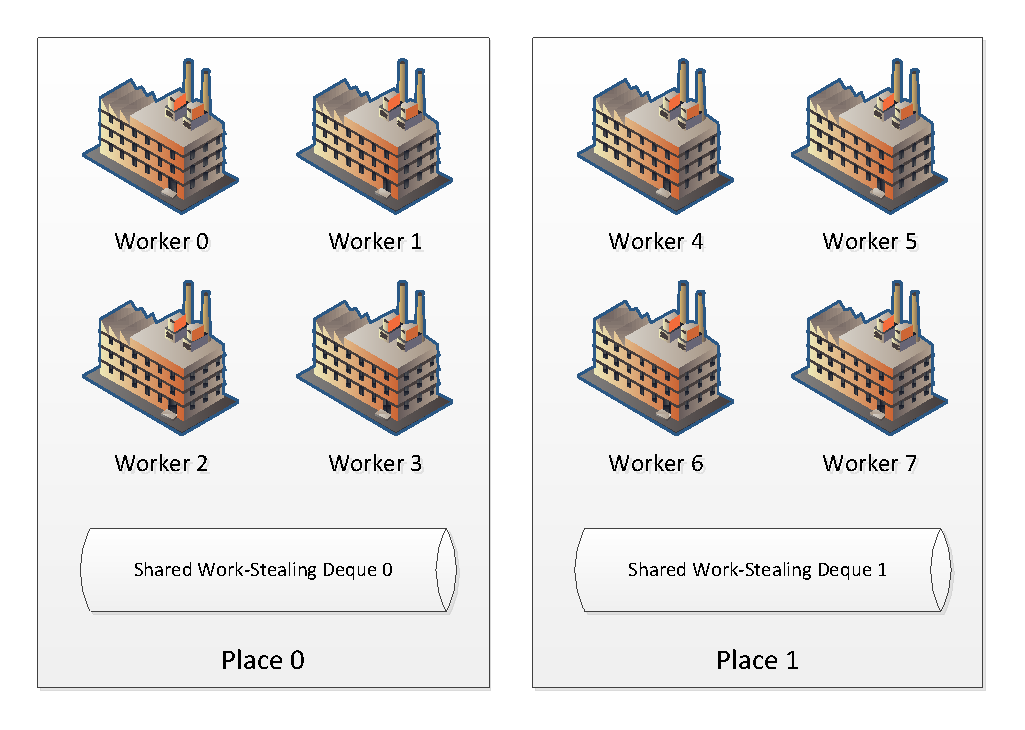
\includegraphics[width=\linewidth]{locality-implementation/places}
  \caption{Work-Stealing Places}
  \label{fig:locality-implementation-work-stealing-places}
\end{figure}

Other locality-aware work-stealing schedulers use a more complex
design. \textcite{Acar2000} for example provide each worker with a
mailbox in addition to the work-stealing deque: A mailbox is a FIFO
queue of pointers to work items that have affinity for the worker. So
when creating a work item, a worker will push it onto both the deque,
as in normal work-stealing, and also onto the tail of the mailbox of
the worker that the interval has affinity for. Now a worker will first
try to obtain work from its mailbox before attempting to
steal. Because work items can appear twice, once in a mailbox and once
in a deque, they have to be idempotent (Section
\ref{sec:queues-implementation-idempotent-ws-deque}).

However, we have decided to simplify our scheduler implementation by
using a shared deque per \emph{Work-Stealing Place}. We believe that
this would not impact scalability as long as the places are not too
large. We could show in Section
\ref{sec:queues-performance-single-shared-queue} that up to 8 workers
there is no significant difference between using a separate deque for
each worker or a shared deque per place.

\subsection{Places Implementation}
\label{sec:locality-implementation-work-stealing-places-implementation}

Places are virtual: The mapping of physical units to places is
performed by a concrete implementation of the abstract
\lstinline!Places! class shown in Listing
\ref{lst:locality-implementation-places}.

\lstinputlisting[style=FloatNumbers, 
  caption={Abstract \lstinline!Places! class},
  label=lst:locality-implementation-places]{
    ../listings/locality-implementation/Places.java
}

The abstract \lstinline!Places! class provides a concrete
implementation of the \lstinline!PlaceID! class (Lines
\ref{lst:locality-implementation-places-place-id-start} --
\ref{lst:locality-implementation-places-place-id-stop}) to its
subclasses. 

\emph{Work-Stealing Places} have a couple of public fields and
methods. \lstinline!name! is the name of the place, \lstinline!length!
contains the number of places and \lstinline!unitsLength! saves the
number of overall processing units the machine has. With
\lstinline!getPlaceID()!  we can get a certain place
ID. \lstinline!get()! returns the IDs of the physical units belonging
to a certain place. By calling \lstinline!getUnit()! with the logical
unit ID, we get the physical unit ID.

An example of a concrete place mapping is given in Listing
\ref{lst:locality-implementation-mafushi-places}. The class
\lstinline!NehalemPlaces! defines the places for our Intel Nehalem
test machine according to its memory hierarchy. As Figure
\ref{fig:locality-implemenation-work-stealing-places-mafushi} depicts
this system includes two processors with four cores each. The machine
has 12 GB RAM and both processors have a direct connection to half of
the memory space. While every core has its separate level 1 and level
2 caches, the per-processor 8 MB level 3 cache is shared between all
cores of the same processor.

\lstinputlisting[style=FloatNumbers, 
  caption={Places configuration for Intel Nehalem in a two-processor configuration},
  label=lst:locality-implementation-mafushi-places]{
    ../listings/locality-implementation/NehalemPlaces.java
}

We define a place for each processor (Lines
\ref{lst:locality-implementation-mafushi-place-ids-start} --
\ref{lst:locality-implementation-mafushi-place-ids-stop}). Place 0
consists of the physical units 0, 2, 4, and 6 (Line
\ref{lst:locality-implementation-mafushi-place-0}) and the physical
units 1, 3, 5, 7 belong to place 1 (Line
\ref{lst:locality-implementation-mafushi-place-1}). Line
\ref{lst:locality-implementation-mafushi-places-units} defines the
mapping of the virtual units to the physical processing units.

\begin{figure}[!htb]
  \centering
  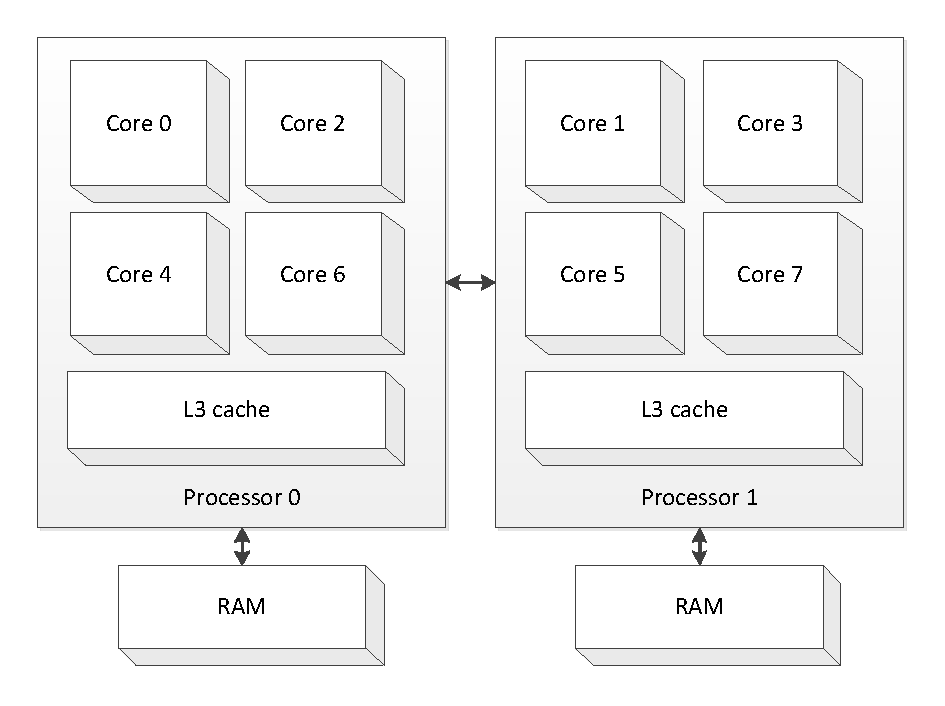
\includegraphics[width=0.92\textwidth]{locality-implementation/mafushi}
  \caption[Intel Nehalem in a two-processor configuration]{Intel
    Nehalem in a two-processor configuration}
  \label{fig:locality-implemenation-work-stealing-places-mafushi}
\end{figure}

\subsection{Scheduling Policy}
\label{sec:locality-implementation-work-stealing-places-scheduling}

When an interval is ready to run, we first get its place ID. If the
place ID is \lstinline!null!, i.e. the interval is locality-ignorant,
we either enqueue it at the place of the currently active worker or
add it at a place in a round-robin fashion. If a place ID is given,
then the interval is locality-aware and we enqueue it at the specified
place.


\section{Setting Core Affinity of Worker Threads}
\label{sec:locality-implementation-core-affinity}

In recent Java Virtual Machines, threads are implemented with native
threads. A Java program using threads is no different from a native
program using threads, i.e. a Java thread is just a native thread
belonging to a JVM process. This means there is a 1-to-1
correspondence between Java and native threads. When using the GNU C
library on Linux, native threads are implemented with the NPTL (Native
POSIX Threads Library). NPTL is also a 1-to-1 implementation, meaning
that each thread maps to a kernel scheduling entity. Figure
\ref{fig:locality-implementation-core-affinity-thread-mapping}
illustrates this 1-to-1 thread mapping.

\begin{figure}[htb]
  \centering
  \begin{tikzpicture}
    [node distance=0.8cm,
    start chain=going below,]
    \node[box, join] {Java Thread};
    \node[box, join] {Native POSIX Thread};
    \node[box, join] {Kernel Scheduling Entity};
  \end{tikzpicture}
  \caption{Linux 1-to-1 thread mapping}
  \label{fig:locality-implementation-core-affinity-thread-mapping}
\end{figure}

Unfortunately the Java Threads API does not expose the ability to set
the CPU or core affinity despite numerous use cases where setting the
affinity of threads would be beneficial -- such as improving cache and
network performance or real-time applications \cite{Love2003, Dow2005,
  Foong2008}. There exists a request for enhancement on this issue but
it was set to the state \emph{``Closed, Will Not Fix''}
\cite{Oracle1999}.

\subsection{JNI Library}
\label{sec:locality-implementation-core-affinity-jni-library}

To bind the workers to a specific core, we wrote a small JNI library
-- see Listing \ref{lst:locality-implementation-core-affinity} for the
API. The method \lstinline!set(int physicalUnit)!  (Line
\ref{lst:locality-implementation-core-affinity-set-unit}) is used to
bind the current thread to a physical unit. With
\lstinline!set(int[]physicalUnits)! the current thread can be bound to
several physical units, for example to a node in a NUMA system (Line
\ref{lst:locality-implementation-core-affinity-set-node}). The workers
of the intervals scheduler use \lstinline!set(int physicalUnit)! in
their \lstinline!run()! method to set the affinity to a separate
physical unit each.

\lstinputlisting[style=FloatNumbers,
  caption={\lstinline{Affinity} class with interface for the native methods}, 
  label=lst:locality-implementation-core-affinity]{
    ../listings/locality-implementation/Affinity.java 
}

Listing \ref{lst:locality-implementation-core-affinity-jni-header}
contains the native method declarations which are implemented in
Listing \ref{lst:locality-implementation-core-affinity-jni-set}. Line
\ref{lst:locality-implementation-core-affinity-jni-h-set-unit}
declares \lstinline!set(int physicalUnit)! and on Line
\ref{lst:locality-implementation-core-affinity-jni-h-set-node} we
declare the method \lstinline!set(int[] physicalUnits)!.

\lstinputlisting[style=FloatNumbersC, 
  caption={\lstinline{Affinity} class: JNI C header}, 
  label=lst:locality-implementation-core-affinity-jni-header]{
    ../listings/locality-implementation/ch_ethz_hwloc_Affinity.h 
}

\lstinputlisting[style=FloatNumbersC, 
  caption={\lstinline{Affinity} class: JNI C implementation to set the affinity},
  label=lst:locality-implementation-core-affinity-jni-set]{
    ../listings/locality-implementation/ch_ethz_hwloc_Affinity_set.c 
}

The implementation for setting the affinity is shown in Listing
\ref{lst:locality-implementation-core-affinity-jni-set}. When setting
the affinity, we first initialize the CPU set structure (Lines
\ref{lst:locality-implementation-core-affinity-jni-set-unit-init-cpuset}
and
\ref{lst:locality-implementation-core-affinity-jni-set-node-init-cpuset})
and then we set it to the specified physical units (Lines
\ref{lst:locality-implementation-core-affinity-jni-set-unit-set-cpuset}
and
\ref{lst:locality-implementation-core-affinity-jni-set-node-set-cpuset}). The
actual affinity change is carried out in function
\lstinline!set_affinity()! on Lines
\ref{lst:locality-implementation-core-affinity-jni-set-impl-start} --
\ref{lst:locality-implementation-core-affinity-jni-set-impl-end}.

Before we can set the affinity of a Java thread, we need to get its
native thread ID. To get the native thread ID, we use the
\lstinline!pthread_self()! function (Line
\ref{lst:locality-implementation-core-affinity-jni-set-impl-pthread-self}). The
function \lstinline!pthread_setaffinity_np()! (Line
\ref{lst:locality-implementation-core-affinity-jni-set-impl-set}) sets
the CPU affinity mask of the thread to the CPU set pointed to by
\lstinline!cpuset!.  If the call is successful, and the thread is not
currently running on one of the CPUs in \lstinline!cpuset!, then it is
migrated to one of those CPUs. If there is an error,
\lstinline!pthread_setaffinity_np()!  returns a nonzero error number
and we throw an exception (Line
\ref{lst:locality-implementation-core-affinity-jni-set-impl-set-error}).

\subsection{Restrictions}
\label{sec:locality-implementation-core-affinity-restrictions}

\subsubsection{Portability}

As we are directly using functions provided by POSIX threads, our
implementation is not portable across operating systems that do not
support the POSIX standard. To make our library portable, it could be
rewritten using \emph{Portable Linux Processor Affinity (PLPA)}
\cite{OpenMPI2010a} or \emph{Portable Hardware Locality (hwloc)}
\cite{OpenMPI2010}.

\subsubsection{Data Locality}

By setting the core affinity of threads, we only control the locality
of the work but we do not have control over data locality.

In a NUMA system every node has a direct connection to local memory
providing fast access, and an indirect connection to remote memory
with slower access. In the Intel Nehalem system for example, local
DRAM access takes $\sim 60$ ns, while remote DRAM access takes $\sim
100$ ns (Table \ref{tab:locality-introduction-memory-access-times}).

In the Java HotSpot VM, the NUMA-aware allocator has been implemented
to provide automatic memory placement optimizations for Java
applications \cite{Masamitsu2008, Oracle2010, Humble2010}: The
allocator controls the eden space of the young generation of the heap,
where most of the new objects are created. It divides the space into
regions each of which is placed in the memory of a specific node. The
allocator relies on a hypothesis that a thread that allocates the
object will be the most likely to use the object. To ensure the
fastest access to the new object, the allocator places it in the
region local to the allocating thread.

On Linux, the implementation is based on work by
\textcite{Kleen2004}. To enable the NUMA-aware allocator, we have to
invoke the JVM with the parameter \verb!-XX:+UseNUMA!.


%%% Local Variables: 
%%% mode: latex
%%% TeX-master: "thesis"
%%% End: 
